\chapter{Evaluation and Results}
\label{ch:evaluation-and-results}

\section{Data Analysis}
\label{sec:data-analysis-evaluation}

    % This section contains analysis of the data 
% \section{Introduction}
\section{Evaluation Setup}
\label{sec:evaluation-setup}
% How everything was set up (kubernetes, ml,...)

  In this section the evaluation setup will be described in detail. 
  This involves what tools and technologies were used and how they were combined in order to evaluate our test cases. Additionally, the \nameref{sec:forecasting-metrics-evaluation-setup} that are used are briefly described since they are crucial for the forecast prediction performance comparisons.
  
  \subsection{Hardware}
  \label{sec:hardware}

    The training of the \nameref{sec:lstm-background} model was done on a GPU server provided by ITEC, University Klagenfurt. The server specifications are as follows:

    \begin{center}
      \begin{tabular}{| l | l |}
        \hline
        \textbf{Processor}   &   Intel Xeon Gold 5218 CPU @ 2.30GHz (64 cores) \\ \hline
        \textbf{GPU}         &   2 x NVIDIA Quadro RTX 8000 GPU (48 GB RAM)    \\ \hline
        \textbf{Main Memory} &   754 GB                                        \\ \hline
        \textbf{Operating System} &  Ubuntu Linux 18.04 LTS                    \\ \hline

        \hline
      \end{tabular}
      \end{center}

  \subsection{Docker}
  \label{sec:docker-evaluation-setup}

    Docker is an open-source platform for automating the deployment of applications inside containers. A container is a standalone executable package that includes everything needed to run a piece of software, including the code, runtime, libraries, environment variables, and system tools.
    Abstracting applications as containers provide a consistent and reproducible environment, which makes it easier to move applications between development, testing and production environments.
    Containers are often used to package an entire application with all it's dependencies into a single container image that can easily be moved and run on any device with a Docker runtime.
    The docker toolbox provides tools for building, shipping and running containers, including a runtime environment for containers called Docker Engine, Docker Hub (a repository for storing and sharing images) and the Docker CLI to be able to interact with Docker via a command-line interface.

  \subsection{Kubernetes}
  \label{sec:kubernetes-evaluation-setup}
    Kubernetes is an open-source platform for automating deployment, scaling, and management of containerized applications. It was originally developed by Google and is now maintained by the Cloud Native Computing Foundation (CNCF).
    Kubernetes provides a way to manage and organize containers (such as \nameref{sec:docker-evaluation-setup} containers) at scale, making it easier to deploy, update, and maintain applications. It does this by abstracting the underlying infrastructure and providing a unified API for managing containers.
    Kubernetes helps to automate many of the manual tasks involved in deploying and managing containers, such as scaling up or down the number of replicas of an application, rolling out updates, and managing network and storage resources. It also provides features for scaling and self-healing, allowing your applications to be more robust and resilient.
    Kubernetes has become a popular platform for deploying cloud-native applications and is widely used by organizations of all sizes across various industries.

  \subsection{NetData}
  \label{sec:netdata-evaluation-setup}

    Netdata is an open source tool that collects real-time metrics, including CPU usage, disk activity, bandwidth usage and further more.
    The reason we chose Netdata for monitoring is that it is a lightweight tool mostly written in C, Python and Javascript and it requires minimal resources, which is necessary when monitoring edge devices.
    One of its major features is that it runs without interrupting any of the applications running on the same device. This is achieved by only using idle CPU cycles while running.
    Netdata provides an in-browser dashboard to analyse each metric in real time with help of visual representation. As an example, a screenshot was taken of a cloud resource in our system as can be seen in \ref{fig:netdata-dashboard}.
    \begin{figure}[h!]
        \centering
        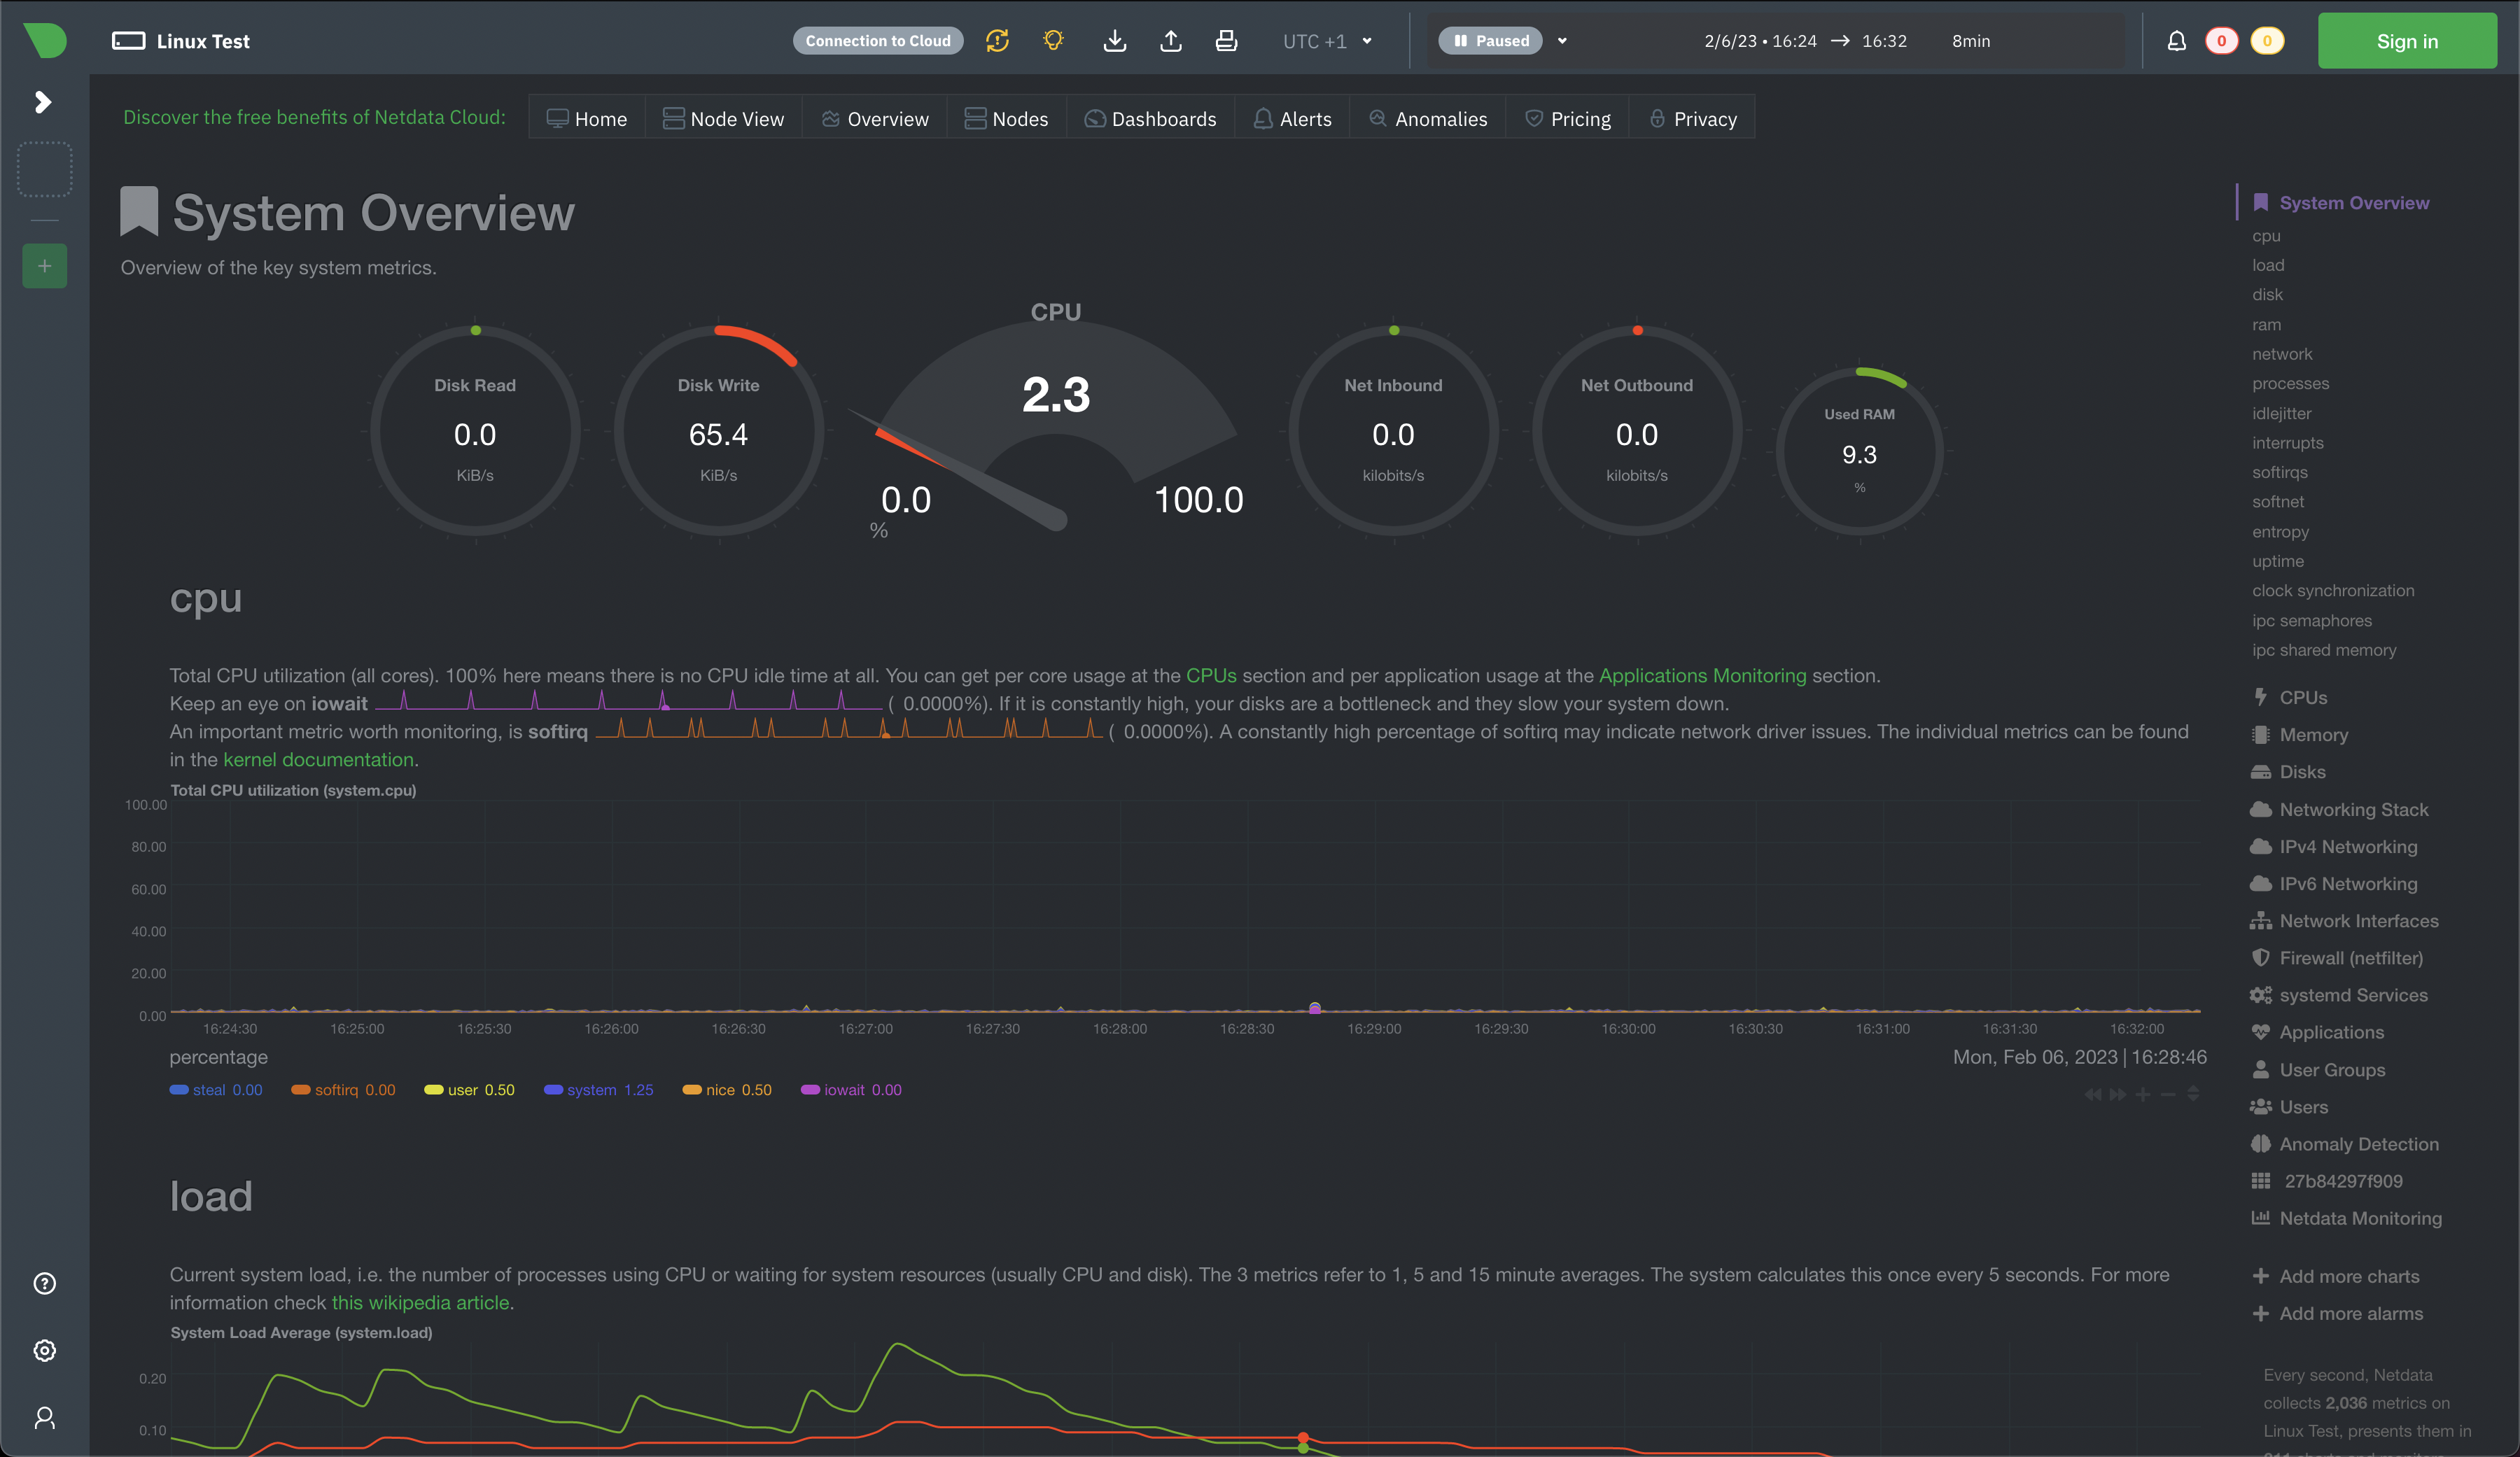
\includegraphics[width=0.95\textwidth]{figures/netdata.png}
        \caption{Netdata Dashboard Example}
        \label{fig:netdata-dashboard}
    \end{figure}
    Netdata has a vast amount of support for other tools in order to gather data. 
    One of the supported tools is \nameref{sec:prometheus-evaluation-setup}, which is used to scrape the monitored data from all resources that have Netdata installed.

  \subsection{Prometheus}
  \label{sec:prometheus-evaluation-setup}
  
    Prometheus\footnote{https://prometheus.io/} is an open source application used for monitoring and alerting of events and is designed to run across various platforms in a scalable and easily deployable manner.
    Same as Netdata it records in real-time, and stores the gathered metrics in a time series database by using a \emph{HTTP pull model}. It also allows real-time alerting via a rule defining configuration and also has a flexible query language called \emph{PromQL}, that enables the retrieval and processing the gathered data. Prometheus has great integration with other tools such as Netdata.
    In the project it is used inside a monitoring master node that is continuously scraping all resources that have Netdata installed for monitoring data. In case a predefined rule is broken at a monitored resource, such as CPU over-allocation, Prometheus triggers an event that notifies ADA-PIPE in order to be able to take measurements.

  \subsection{PyTorch}
  \label{sec:pytorch-evaluation-setup}
    PyTorch\footnote{https://pytorch.org/} is an open-source machine learning library for Python, developed by Facebook's AI Research lab (FAIR). It provides tensor computation (similar to NumPy) with strong support for deep neural networks built on a tape-based autograd system. PyTorch is designed to provide flexibility and ease of use, with a focus on deep learning and neural networks. It can be used for various tasks such as natural language processing, computer vision, and speech recognition.
    PyTorch also supports deployment on various platforms, including CPUs, GPUs, and TPUs, and has an active community of users and contributors that continue to improve and expand its capabilities.
  

  \subsection{LSTM Model Setup}

  \subsection{LSTM Hyperparameters}
  \label{sec:lstm-hyperparameters-evaluation-setup}


  \subsection{Weights \& Biases}
  \label{sec:wandb-evaluation-setup}
    
    Weights \& Biases (W\&B)\footnote{https://wandb.ai} is a software company that provides an AI platform for machine learning and deep learning. Their platform provides tools for tracking experiments, visualizing models, and collaborating with team members.
    The platform provides a centralized repository for all of the information related to a machine learning project, including code, data, models, and results.
    W\&B offers a range of features to help users better understand their models, including interactive visualizations of model architecture, weight distributions, and training metrics. The platform also provides a suite of tools for tracking experiments, which makes it easy to compare different models and understand the impact of changes to the code or data.

    % The W\&B platform is designed to make it easier for data scientists, machine learning engineers, and researchers to manage the complexity of developing and deploying machine learning models. 


    % Overall, W\&B provides a comprehensive solution for machine learning and deep learning development, and can be a valuable tool for organizations looking to streamline their machine learning operations and improve their ability to develop high-quality models.
  
  \subsection{Forecasting Metrics}
  \label{sec:forecasting-metrics-evaluation-setup}

    Forecasting metrics \cite{botchkarevPerformanceMetricsError2018} are measures used to evaluate the accuracy of forecasting models. These metrics are used to compare different models, assess the quality of the forecasts, and identify areas for improvement.

    % Maybe add those metrics? 

    % Mean Absolute Error (MAE): measures the average magnitude of the error between the predicted values and the actual values.

    % Theil's U-Statistic: measures the accuracy of a forecast relative to the accuracy of a naive forecast.

    % Mean Absolute Scaled Error (MASE): measures the accuracy of a forecast relative to the accuracy of a naïve forecast.

    The choice of forecasting metric will depend on the specific goals and requirements of the forecasting task. Some metrics may be more appropriate for certain types of data or models, while others may be better suited for comparing different models.
    Overall, the use of appropriate forecasting metrics is critical for evaluating the accuracy of forecasting models and for identifying areas for improvement.

    \paragraph{MAPE}
    \label{par:mape-metrics-evaluation}
      Mean Absolute Percentage Error (MAPE) \cite{demyttenaereMeanAbsolutePercentage2016} is a commonly used metric for evaluating the accuracy of forecasting models. It measures the average percentage difference between the predicted values and the actual values.
      The formula for MAPE is:

      \begin{definition}{Mean Absolute Percentage Error}
        $$MAPE = \frac{1}{n} \times \sum \left|\frac{Actual - Predicted}{Actual}\right| \times 100$$
      \end{definition}
      where $n$ denotes the number of data points and $Actual$ and $Predicted$ are the actual and predicted values, respectively.
      MAPE provides a percentage error, which makes it easy to interpret and compare the accuracy of forecasting models. 
      
      However, there are some limitations to using MAPE, such as the fact that it can become undefined when the actual value is zero (in our case if there is no resource utilisation at some time step $i$), and it can be sensitive to outliers.
      Despite these limitations, MAPE is a widely used metric for evaluating forecasting models, especially if it is important to understand the relative magnitude of the errors in the predictions. 
      Overall, MAPE provides a useful way to measure the accuracy of forecasting models and can help to identify areas for improvement in the model or the data.


    \paragraph{sMAPE}
    \label{par:smape-metrics-evaluation}
    
      Symmetric Mean Absolute Percentage Error (SMAPE) \cite{kreinovichHowEstimateForecasting2014} is a metric used for evaluating the accuracy of forecasting models. It measures the average percentage difference between the predicted values and the actual values, and is symmetrical in that it treats positive and negative errors equally.
      In our evaluation of the prediction performance this is especially useful since both over-, and under-utilisation are present in all prediction variants.
      The formula for SMAPE is:

      $$sMAPE = \frac{1}{n} \times \sum \left|\frac{Actual - Predicted}{\left(Actual + Predicted\right) \div 2}\right| \times 100$$
      where $n$ denotes the number of data points and $Actual$ and $Predicted$ are the actual and predicted values, respectively.
      sMAPE provides a percentage error similar to \nameref{par:mape-metrics-evaluation}, which makes it easy to interpret and compare the accuracy of forecasting models. Unlike MAPE, sMAPE is symmetrical, since it doesn't become undefined when the actual value is zero, and another difference is that it is less sensitive to outliers.
      Overall, sMAPE is a useful metric for evaluating the accuracy of forecasting models and can provide valuable information for understanding the relative magnitude of the errors in the predictions.

    \paragraph{RMSE}
    \label{par:rmse-metrics-evaluation}

      Root Mean Square Error (RMSE) \cite{chaiRootMeanSquare2014} is a metric used for evaluating the accuracy of forecasting models. It measures the average magnitude of the error between the predicted values and the actual values, and provides a useful way to compare the magnitude of the errors in different models.
      The formula for RMSE is:
      $$RMSE = \sqrt{\frac{\sum_{i = 1}^{N}\left(Predicted_i - Actual_i\right)^2}{N}}$$
      where $n$ denotes the number of data points and $Actual$ and $Predicted$ are the actual and predicted values, respectively.
      RMSE provides a measure of the magnitude of the errors in the predictions, with lower values indicating a more accurate model. 
      RMSE is particularly useful when the goal is to minimize the magnitude of the errors in the predictions.
      One important thing to note about RMSE is that it is sensitive to the scale of the data. This means that it is more appropriate to use RMSE when the scale of the actual and predicted values is similar.
      Because of the scale sensitivity of RMSE, the number of actual and predicted values is equivalent for all our evaluation scenarios in order to be able to use RMSE for a comparison between different approaches.
      Overall, RMSE is a widely used and useful metric for evaluating the accuracy of forecasting models and can provide valuable information for understanding the magnitude of the errors in the predictions.

% \paragraph{Theil's U-Statistic}

% Theil's U-Statistic is a measure of the accuracy of a forecasting model relative to a naïve forecast. The naïve forecast is a simple forecast that uses the average or last observed value as the prediction for all future time points. Theil's U-Statistic is used to compare the accuracy of a forecast with the accuracy of the naïve forecast.

% The formula for Theil's U-Statistic is:

% U = (RMSE of the forecast) / (RMSE of the naïve forecast)

% where RMSE stands for Root Mean Squared Error.

% Theil's U-Statistic is a unitless measure, with values ranging from 0 to infinity. A value of 0 indicates that the forecast is no better than the naïve forecast, while a value greater than 1 indicates that the forecast is more accurate than the naïve forecast.

% Theil's U-Statistic is particularly useful when the goal is to compare the accuracy of a forecast with the accuracy of a simple, baseline forecast. It provides a useful way to evaluate the improvement in accuracy achieved by using a more sophisticated forecasting model.

% Overall, Theil's U-Statistic is a valuable tool for evaluating the accuracy of forecasting models, and for comparing the accuracy of different models relative to a simple, baseline forecast.
    \paragraph{Resource Wastage}
    \label{par:resource-wastage-metric-evaluation}
      Calculated by subtracting the surface area of allocated - predicted.

\section{Evaluation Scenarios}
\label{sec:evaluation-scenarios}

% the different evaluations I did like task type or batch size
% what is common in the scenarios (or some of them)
    In the evaluation scenarios 1-4, the forecast performance of different machine learning training scenarios is evaluated and compared with each other. Each of them builds on top of the previous evaluation scenario to compare the improvement.

  \subsection{1. Simple Feature Set}
  \label{sec:simple-feature-set-evaluation-scenarios}
    
    The simple feature set denotes a \nameref{sec:lstm-background} model that was trained with a feature set that only contains the allocated CPU and memory a user provided for the submitted task as well as the capacity of the worker pool resource the task should be deployed to. Additionally, since LSTMs are designed to handle sequential data, the order of the incoming tasks is also an important information for the model, and thus cannot be randomized as is common for other machine learning algorithms.

  \subsection{2. Adding Task Knowledge}
  \label{sec:adding-task-knowledge-evaluation-scenarios}

    In this evaluation scenario, the feature set used to train the LSTM model contains additionally to the feature set arguments of the \nameref{sec:simple-feature-set-evaluation-scenarios} also \emph{task knowledge}. This task knowledge refers to the type a task is classified as. The task knowledge was first extracted from the data set and transformed with the \emph{one-hot encoding} \cite{husseinEnhancementPerformanceRandom2021} method. One-hot encoding adds a feature vector to the feature set consisting of $0$ and $1$, where $1$ denotes the type of a task, and the rest of the vector values are $0$ for that task. This technique is useful when categorical data should be fed to a machine learning model since many model architectures can only handle numerical values, making it necessary to transform strings or other data types to numbers.
    \begin{quote}
      One hot encoding is a process of converting categorical data variables so they can be provided to machine learning algorithms to improve predictions. \emph{One hot encoding is a crucial part of feature engineering for machine learning.} \cite{fawcettDataScienceMinutes}
    \end{quote}
    The additional information about the task type enables the LSTM model to better discern the actual utilisation that is required for each task.
    The task knowledge also provides information regarding the order of tasks, since patterns of reoccurring tasks also help the model to generate more accurate predictions in theory.

    \paragraph{CPU Prediction Evaluation}
    \label{par:cpu-prediction-evaluation-task-knowledge}

      Providing categorical data is able to positively influence the prediction performance of the machine learning model. This is also seen in the predictions of our LSTM model. The additional knowledge about what type of tasks are present in the pipeline enabled the ML model to create more accurate predictions of the CPU utilisation for each task.

      As can be seen in the figure 
      % \ref{fig:cpu-comparision-no-tasks-vs-tasks} 
      the CPU utilization could be predicted more accurately if the model was trained with the additional information about which type of task will be allocated onto the system.
      Compared to the ML model trained without this additional knowledge (further on called NT-model, short for No-Tasks-model), the model trained with task knowledge is able to predict the required allocation on a finer granularity.
      This is observed in the predictions as more changes in the prediction values occur compared to the NT-model, which often seems to predict an average value over a greater time span rather than predicting the allocation for each task itself.
      The WT-model is also more sensitive to great utilization spikes and periods of utilization close to zero compared to the NT-model.

    \paragraph{Memory Prediction Evaluation}
    \label{par:memory-prediction-evaluation-task-knowledge}

      Similar to the prediction of the CPU utilization, the memory utilization was improved if the ML model was trained with additional information about the task type. This enabled the model to achieve more a accurate prediction of the actual memory usage compared to the NT-model.

      This improvement is even more apparent compared to the allocated memory data which heavily over-allocated the required amount of memory. Compared to the NT-model and allocated memory the WT-models predictions are able to reduce the gap between predicted memory utilization and actual memory utilization the furthest.

  \subsection{3. Adding Instance Knowledge}
  \label{sec:adding-instance-knowledge-evaluation-scenarios}

    In this evaluation scenario, the feature set used to train the LSTM model contains additionally to the feature set arguments of the \nameref{sec:adding-task-knowledge-evaluation-scenarios} also information about the number of instances that are required to be deployed. While the knowledge about the number of instances is similarity one-hot encoded as is the task knowledge (see \ref{sec:adding-task-knowledge-evaluation-scenarios}), adding one feature vector column for every instance number would have resulted in exploding the feature data set with 800 additional columns, since the minimum instance number is $1$ and the maximum is $800$.
    For this reason, the feature vector for the one-hot encoded instances were first clustered into $10$ buckets in $50$ iterations by k-means clustering \cite{hartiganAlgorithm136Kmeans1979}.

  \subsection{4. Training with Custom Loss Function}
  \label{sec:training-with-custom-loss-function-evaluation-scenarios}

      As discussed in the previous evaluation scenarios, 
      additional information regarding a task (see sections \ref{sec:adding-task-knowledge-evaluation-scenarios} and \ref{sec:adding-instance-knowledge-evaluation-scenarios}) will result in closer predictions to the actual value but also the LSTM model is more likely to predict values that are smaller than the actual value.
      % TODO explain why this is a bad thing
      
      Therefore, a custom loss function was designed and implemented (see \nameref{sec:penalty-mse-loss-function-architecture-and-implementation}) to counter the prediction of values lower than the actual value.

  \subsection{5. Inference Time}
  \label{sec:inference-time-evaluation-scenarios}

    The evaluation scenario regarding the inference time measures the time that is required for the LSTM model to forward a prediction.
    The time measurement is done on different batch sizes. This is important to be able to forward the resource utilisation prediction to the scheduler in an acceptable time frame.


  \subsection{6. Prediction Performance depending on Batch Size}
  \label{sec:prediction-performance-depending-on-batch-size-evaluation-scenarios}



    % Different batch sizes
    % Different models?



  The batch size not only influences the required training time and  on how much sampling data at once the model weights are updated on. The used batch size even has an impact on the prediction performance of the LSTM model.
    
  As can be seen in figure 
  % \ref{fig:comparison-of-500-1000-batch-size}, 
  
  the batch size used while training the LSTM model has significant impact on the overall prediction performance.
  In the figure, the training batches have the sizes 500 (orange dashed line) and 1000 (blue dashed line) elements per batch, the actual CPU utilization is shown as the black line and the CPU cores (in percent) allocated by the user are shown in the green line. While the prediction with a batch size of 500 did overestimate the CPU utilization, it has some great prediction results in the largest utilization spike, where it did come closest to the actual CPU utilization and also corrected the CPU allocation in multiple instances to either correctly use less or more CPU cores for a task.
  
  % The training was done on a dataset size of 4000 elements total, which is only a small fraction of the actual dataset size.
  
  
  % \begin{figure}[h!]
  %     \centering
  %      \includegraphics[width=\columnwidth]{figures/500_1000bs_comparison.png}
  %     \caption{CPU Comparison of Batch Sizes 500 and 1000 - Part 1}
  %     \label{fig:comparison-of-500-1000-batch-size}
  % \end{figure}


  In figure 
  % \ref{fig:comparison-of-500-1000-batch-size-2},
   it is shown that the model with a batch size of 1000 is more accurately predicting lower utilization values and its overall bias in the dataset is to predict lower utilization values.
  The model trained with batch size 500 predicts a higher CPU utilization in general, but also did correctly increase/decrease the CPU utilization if the actual utilization was high/low for a longer period of time.

  The opposite is observed for the model with batch size 1000. 
  This model is more accurate in predicting short utilization spikes or declines compared to the model with a batch size of 500.
  
  % \begin{figure}[h!]
  %     \centering
  %      \includegraphics[width=\columnwidth]{figures/500_1000bs_comparison2.png}
  %     \caption{CPU Comparison of Batch Sizes 500 and 1000 - Part 2}
  %     \label{fig:comparison-of-500-1000-batch-size-2}
  % \end{figure}


  In figure 
  % \ref{fig:comparison-of-500-1000-batch-size-mem}, 
  the prediction of the memory utilization is shown.
  Opposed to the CPU utilization prediction, in the model trained with the smaller batch size is biased to predict lower values in general, and the model trained with a batch size of 1000 predicted higher utilization values. Also it was able to produce accurate predictions of the memory utilization of tasks.
  \subsection{7. Machine-Sorted vs. Time-Stamp-Sorted Data}
  \label{sec:machine-sorted-vs-time-stamp-sorted-data-evaluation-scenarios}

    
% \section{Monitoring}



\section{Adaptation}
